\chapter{Discussion}

This chapter discusses the resulting city generation software, CityCraft, from three different perspectives.
First, the quality of the application and the city models it generates are estimated by addressing the checklist that was presented at the end of Chapter \ref{section:goal_and_scope}.
This perspective also argues how the choice of different algorithms could have affected the results.
Subsequently, the validity of the processes used during development is debated.
Finally, the last subchapter discusses further research.

% Ended up being a bit more about 3D graphics than intended, but that proved intresting challenges as well.

\section{Quality of Results}

As described in~\ref{section:goal_and_scope}, the quality of the generated city is difficult to measure objectively.

% Do models correctly integrate with third-party software such as Blender \cite{blender}?
\textbf{Q1}:
The generated models imports correctly into Blender~\cite{blender}.
Integration with other third-party tools however, would have to be tested more thoroughly as Blender was the main tool used for testing exported models could be imported correctly to an external tool. 

Although the 3D models are imported correctly in terms of their model data there exists some unintended visual differences.
These differences are however, a consequence of the different rendering pipelines between Unity and any other third-party tool.
Figure~\ref{fig:blender_shading_result} showcases these visual differences in Blender.

% TODO(anton): Add Figure of resulting model imported into blender
% \begin{figure}[h!]
%   \centering
%   \includegraphics[width=1\textwidth]{figure/discussion_blender_import}
%   \caption{Visual differences between Unity and Blender of a generated city.}
%   \label{fig:blender_shading_result}
% \end{figure}

Importing a generated city into Blender also takes a substantial amount of time in comparison to when exporting the files from within CityCraft.
The importing can take up to 5 minutes on a modern desktop computer.

In conclusion, the integration with third-party software such as Blender works albeit with some frustration.

% How well is the codebase structured for replacement and expansion of features?
\textbf{Q2}:
Another aspect that was considered was how well the codebase structured for replacement and expansion of new features.
As the generation is divided into a number of sub-generators it would be easy to add more generators on to the total generation.
Furthermore, the generators themselves are structured in a way that adding more content to them, or modifying them should be a simple adaptation to make. 

Implementing more complicated features that has to alter previously generated content is however one limiting factor.
For example, a feature that was of interest was to create road entrances that lead into parking lots.
This feature was however difficult to implement as accessing and creating a junction in the previously generated road network might alter some intermediate generation steps and break the function-based architecture.

% How much notable variety is there in the generated content?
\textbf{Q3}:
When discussing the variety of the generated cities the group distinguished between the overarching structural variety and the variety in textures and shapes of the content.
In terms of the topological structure or layout of the generated cities the group is content with the variety offered.
Each city has a unique look and vary in their size and layout in a way that the group considers realistic enough.
This variety is showcased in Figure~\ref{fig:discussion_city_layout_variety}.

\begin{figure}[h!]
  \centering
  \begin{subfigure}[b]{0.455\textwidth}
    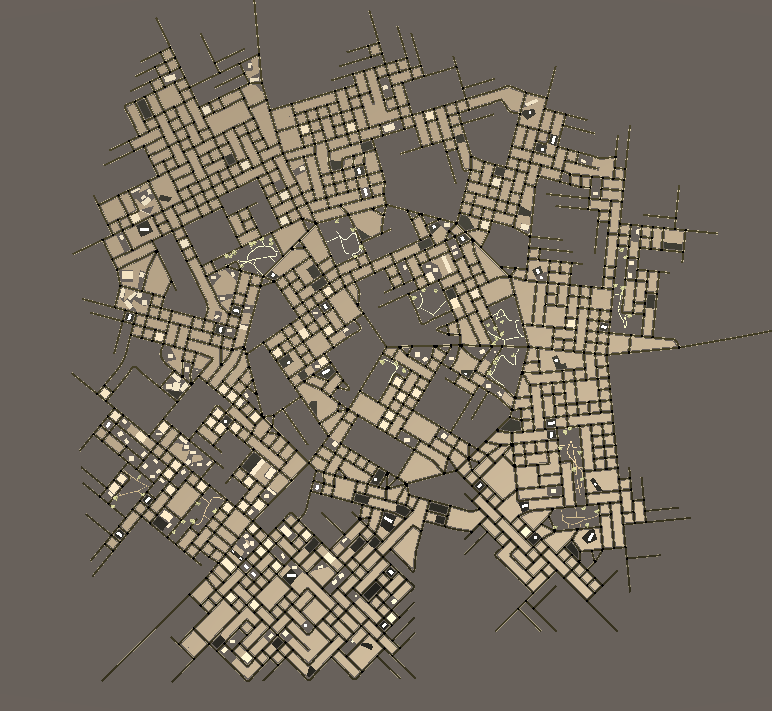
\includegraphics[width=\textwidth]{figure/discussion_city_layout_1}
  \end{subfigure}
  \quad
  \begin{subfigure}[b]{0.45\textwidth}
    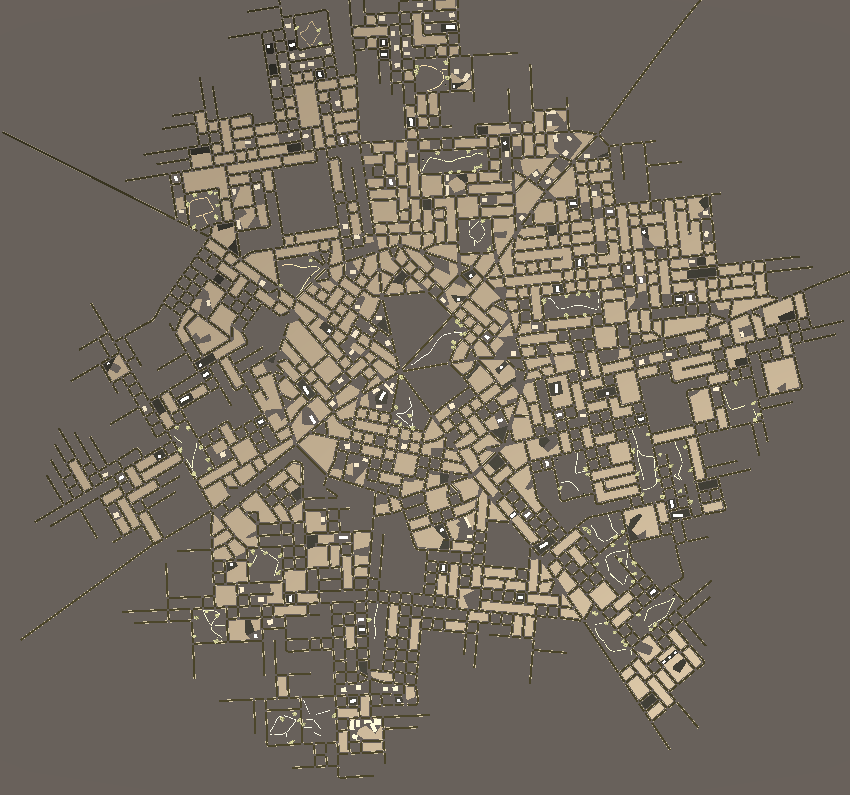
\includegraphics[width=\textwidth]{figure/discussion_city_layout_2}
  \end{subfigure}
  \caption{Cities generated after two consecutive runs under the same conditions highlighting the structural variety.}
  \label{fig:discussion_city_layout_variety}
\end{figure}

The variety in textures and shape variety of skyscrapers, buildings and roads are however limited.
Roads for example, always have the same appearance in terms of their cross-section and texture.

% How much control do the users have over the generation?
\textbf{Q4}:
% TODO(anton): find other description than seed-based
The degree of control offered to the user is, with a few exceptions, at the level of supplying static settings to each subgenerator.
The exception to this is that the user can dynamically place individual cities and re-generate the content for each subgenerator.
This distinction highlights an important design choice of either creating a city editor with PCG capabilities or a seed-based city generator capable of producing an infinite world with no dynamic user input whatsoever.
CityCraft, tries to be both in the sense that each subgenerator is essentially seed-based but imposes some user choices in the placement of cities for example.
Since the goal was for CityCraft to be a rough tool for generating cities that designers later could refine, the option for allowing the user to edit specific roads or alter the content of a selected block might not be deemed essential but would nevertheless significantly aid a designer and improve the level of control.

Diving into the controls available to the users.
The user has some varying level of control over the generation at different stages of the generation pipeline.
Terrain generation offers the most options while the city subgenerator offers no parameters to the user. 
Although parameters to some generators are limited the user always has the ability to undo the work of a generator if that has left the user unpleased.

% Are the cities suitable for use in digital media such as games and film?
\textbf{Q5}:
The cities generated by CityCraft are by no means mature enough for use in any production quality digital media.
Some limiting factors for this assessment include the texture quality and unrealistic gaps between the roads and surrounding buildings, parks and parking lots.
The larger flaw resulting from this would be that it would seem impossible for theoretical cars to reach the generated parking lots, without driving on top of the grass that is.
Although, the cities generated might find its use cases as a city template that designers would have to refine by hand.

% Are users without technical expertise able to correctly use the application?
\textbf{Q6}:
When evaluating whether a user without any technical expertise would be able to correctly use the application the group concluded that that is the case.
This was concluded with the reasoning that all implementation details are irrelevant to the user.
Admittedly, the application has not undergone any formal user testing to verify this but since all technical 
The user interface could be improved to provide better feedback to the user.

% Are there any known crashes in the application or visual artifacts in the generated models?
\textbf{Q7}:
There exists some infrequent bugs and crashes that are possible to occur when using CityCraft.
Here, we will cover some of the most critical bugs of the application.

% Placement of cities crash
One known issue is that the placement of cities, under some unknown condition, freezes the application.
This rarely happens but is considered the most critical issue as it completely obstructs the user from using the application.

% Road Walls
Another bug possible is that the mesh generated for road intersections can become huge and cover half the world.
The cause for this is known, however due to the time limit hasn't been addressed properly.
% TODO: add figure?



\section{Process and Workflow}

One main takeaway from this project was that even though we believed our defined scope was reasonable, we did not take into account how much time one could spend attempting to perfect the parts that were already working.
An area where this became particularly clear was performance.
During the course of the project we would often find the generators creating content which was visually sufficient for what we had hoped to achieve, but the process of generating would be slow. 
The three main parts of the project where we observed that we could increase performance were the following:

\begin{easylist}
  @ Compressing textures.
  @ Decreasing the triangle-count of objects.
  @ Using LOD.
  @ Combining meshes. 
 \end{easylist}
 
The first part of the list was simple to tackle and did not require any additional code to be written, we simply had to alter the resolution at which our textures were imported.
This came from us noticing that the textures were being imported at a very high quality, we could reduce this and still reach almost indistinguishable results visually, and reduce the amount of memory being used drastically. 

The second problem was revealed by the fact that after generating buildings frame rate suddenly became a major concern. 
After inspecting this issue we found that the buildings were being composed of a lot more triangles then they needed and this was fixed by simply the reducing the triangle count. 

% maybe move LOD to road-mesh methods
The third improvement of performance was using LOD.
LOD works by decreasing the visual quality of an object based on some function of the camera distance to that object.
Typically, different distance intervals are configured to corresponding to different quality meshes.
The further away the camera is the lower the quality of the mesh becomes as to improve the efficiency of rendering without a noticeable difference to the user.
In CityCraft, this technique was used extensively for the roads, intersections and buildings and resulted in significantly improved the performance.

The fourth and final major adjustment made for increasing performance was to combine some of our generated meshes. 
Combining meshes for the building generator, when using the L-system strategy, was crucial for lowering memory usage. 
The first version had a mesh for each wall segment, and each wall segment had its material with an accompanying texture. 
The consequence was memory usage peaking over 10GB with a medium-large city. 
There was also the issue with each wall segment was their object spawned into the world.
This object, called GameObject in Unity, has its render, which also meant an increase in the number of batches needed.
Combining the wall segments into one building meant a drastic change in memory usage. 
Only one of each unique material that represented the different wall segments was loaded in Unity.   

Something that could have been utilized more efficiently had we perhaps chosen a more collaborative style when developing our generators rather than dividing them among us, would be re-using already implemented code. 
This became blatantly obvious when working on the path for the parks.
At one part of the project, code was being written for generating meshes for the park paths, while code for doing this had already been written and was being used in the road generation. 
Another problem that arose from this was that the parking lot generator would have probably had to be developed more in collaboration with the road generator in order to find a way to ensure that roads always have an entry to the parking lots.


\section{Future Work}
The areas which was concluded by the group to be of interest when conducting future work was slightly mentioned in the results chapter, however here they are discussed more in depth.

The generation of the terrain could be further developed to include such features as rivers flowing from mountain tops and also having more climates than the ones we stuck with.
This could include such things as massive forests, saharan-like deserts or snow-covered landscapes.
The terrain is currently also not very detailed, which is definitely something that could be worked on. 
As for now, a population map is generated and the user can control its parameters, however the user has no control of its placement. 
Adding the option for the user to mark the population map similarly to how the cities are marked would be a possible feature to enhance the users control. 

The generation of the road network could in practice be worked on infinitely.
By constantly developing new strategies and refining the way the agents work, one could end up generating strategies for each city known to man.
However, a more sensible way to address further working on the road network would be to simply add a couple more strategies, after investigating what more common road networks look like in the real world.
The road network could also be expanded to include road markings, and road signs, and possibly bridges, in order to further mimic the real world.  

Generating buildings is also a task of seemingly endless variety. 
The future work most likely to be adapted here would be to include a larger set of textures, or to algorithmically generate textures in order to further increase the variety of building's appearance while not limiting them to the placement of said textures.
Another area which would be interesting to pursue would be to generate the interiors of the buildings. 
One could also intend to add structures such as airports, churches, police stations, and many many more. 

The park generation could mainly benefit from adding more objects, and finding suitable ways to fit them in the world.
Some such objects were touched on in the method chapter for this generator, but a lot more could be added.
Changes could also be done in size, as well as shape in order to achieve more varying looks. 
One could give some cities each a probability of generating something similar to Hyde Park (London) or Central Park (NYC) which would likely produce some very interesting results.
The path generator was implemented in a way that did not consider concave polygons, this could be solved in a variety of ways by either altering the algorithm for paths, or alternatively, altering the way we divide plots to avoid this entirely. 

The parking lot generation could simply be extended by adding more shapes than the rectangular ones used in this project.


